\documentclass{article}

\usepackage{tikz}
\usetikzlibrary{calc, positioning, shapes.geometric}
\usepackage[dvipsnames]{xcolor}

\usepackage{Sweave}
\begin{document}
\Sconcordance{concordance:jogo-bofsex-nature1.tex:jogo-bofsex-nature1.Rnw:1 6 1 1 0 %
82 1}


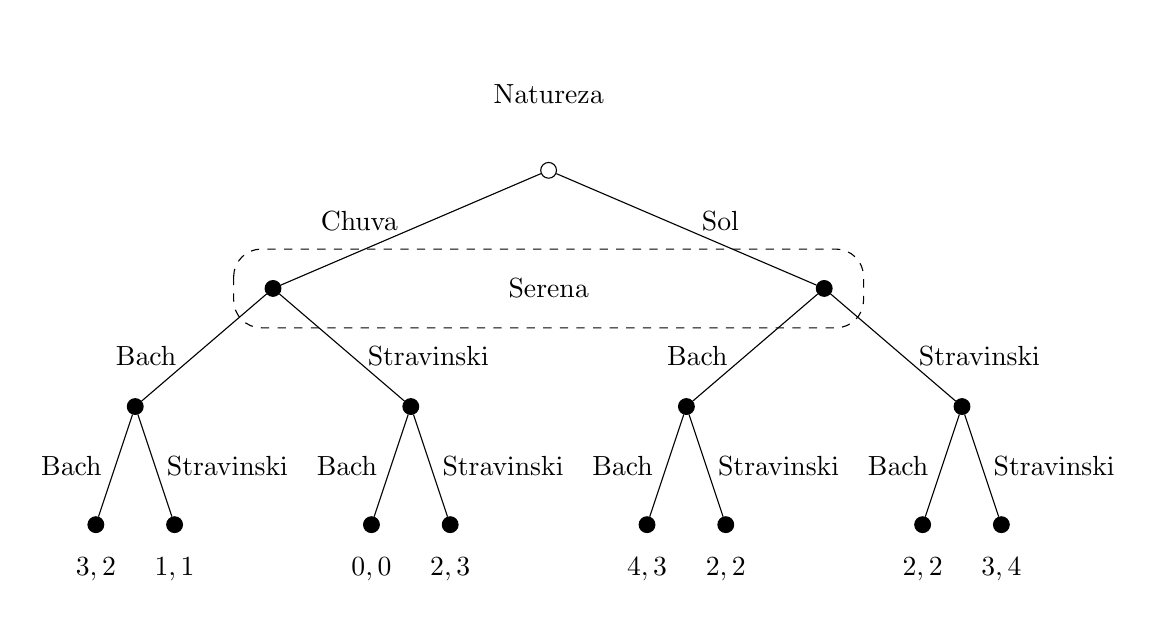
\begin{tikzpicture}[>=stealth, every node/.style={circle}]
\tikzstyle{solid node}=[draw, circle, fill=black, inner sep=1.5, minimum size=2mm]
\tikzstyle{hollow node}=[draw, circle, inner sep=1.5, minimum size=2mm]
\tikzstyle{decision}=[draw, rectangle, fill=gray!30]
\tikzstyle{level 1}=[sibling distance=70mm]
\tikzstyle{level 2}=[sibling distance=35mm]
\tikzstyle{level 3}=[sibling distance=10mm]

% Natureza moves
\node[hollow node, label=above:{Natureza}] (natureza) {}
  child {node[solid node] (serena1) {}
    child{node[solid node] (nina1) {}
      child{
        node[solid node, label=below:{$3,2$}]{}
        edge from parent
        node[left] {Bach}
      }
      child{
        node[solid node, label=below:{$1,1$}]{}
        edge from parent
        node[right] {Stravinski}
      }
      edge from parent
      node[left, yshift=-3, xshift = -5] {Bach}
    }
    child{node[solid node] (nina2) {}
      child{
        node[solid node, label=below:{$0,0$}]{}
        edge from parent
        node[left] {Bach}
      }
      child{
        node[solid node, label=below:{$2,3$}]{}
        edge from parent
        node[right] {Stravinski}
      }
      edge from parent
      node[right, yshift=-3, xshift = 5] {Stravinski}
    }
    edge from parent
    node[left, yshift=3] {Chuva}
  }
  child {node[solid node] (serena2) {}
    child{node[solid node] (nina3) {}
      child{
        node[solid node, label=below:{$4,3$}]{}
        edge from parent
        node[left] {Bach}
      }
      child{
        node[solid node, label=below:{$2,2$}]{}
        edge from parent
        node[right] {Stravinski}
      }
      edge from parent
      node[left, yshift=-3, , xshift = -5] {Bach}
    }
    child{node[solid node] (nina4) {}
      child{
        node[solid node, label=below:{$2,2$}]{}
        edge from parent
        node[left] {Bach}
      }
      child{
        node[solid node, label=below:{$3,4$}]{}
        edge from parent
        node[right] {Stravinski}
      }
      edge from parent
      node[right, yshift=-3, xshift = 5] {Stravinski}
    }
    edge from parent
    node[right, yshift=3] {Sol}
  };

\node at ($(serena1)!.5!(serena2)$) {Serena};
\draw[dashed,rounded corners=10] ($(serena1)+(-0.5,0.5)$) rectangle ($(serena2)+(0.5,-0.5)$);
\end{tikzpicture}

\end{document}
